\chapter{Implementation}

\section{Architecture}

\begin{figure}[h]
\centering
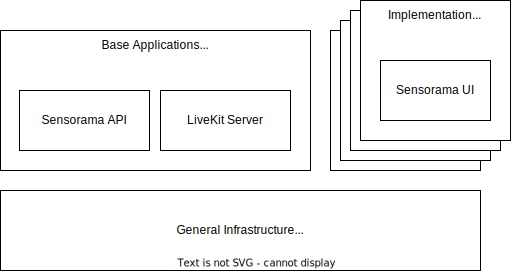
\includegraphics[scale=0.5]{04_Artefakte/01_Abbildungen/sensorama-stack}
\caption[{Sensorama Stack Diagram}]{The main components comprising the application architecture\protect}
\label{fig:sensoramaStack}
\end{figure}

\subsection{Hardware}

The underlying hardware infrastructure is a bare-metal system running on-premises at the university. Due to the containerised packaging and deployment, it could also easily deployed in a cloud environment or other hosting platform. There is no special hardware required and the system could run in any environment that provides network access, storage space and standard computing resources.

In an otherwise containerised application environment, the underlying software infrastructure is minimal. The components required are a Linux \ac{OS}, in this case Ubuntu, with installations of Docker (with ContainerD) and Kubernetes.


\section{Application infrastructure}

While all the frameworks represented in \autoref{fig:mostUsedFrameworks} could be used to build an application as envisioned in this study, Vue is selected as the tool of choice, both due to the relatively high acceptance and the comparably easy learning curve. While it might not be the choice for large-scale or enterprise apps, in this case the low entry barrier and the very simple structure make it ideal to quickly get an app running, experiment with it and pass it on to others for hacking and custom modifications. In order to accelerate and simplify the initial development, the Quasar framework is used as it extends the basic functionality provided by Vue by a \ac{UI} library with layout tools and preset interface elements and a comfortable development and deployment environment.

The choice for a backend framework lands on Feathers and, by extension, Koa. The simple structure and code generators allow for a very quick setup and deployment of a simple WebSockets \ac{API} that provides authentication and resource management. It is connected to a MongoDB database, because there is no stable idea required of how the various resources being stored and retrieved from the database are explicitly structured and typed. With a document store, the data can be easily overwritten with updated data and then wiped before the schema is fixed in place.

LiveKit is chosen as the WebRTC server implementation because it is extremely easy to set up as a container running along the Redis database in Kubernetes. It is extendable, scalable and there is even a hosted variant for people who do not want to run their own server. While Mediasoup would allow a more precise implementation and probably more efficient, the workload overhead for building everything already offered by LiveKit is too much effort for this kind of application. However, it might be interesting to see how components based on Mediasoup could be dropped into this application structure.

\section{Design Paradigms}

The basic design paradigm for the Sensorama application is an \ac{SPA}, 

\subsection{Application Partitioning}

\subsection{Coding Style}

\subsection{Testing}

\section{Application Components}

\subsection{Web Frontend}

\subsection{API Backend}

\subsection{Native Utilities}
